\chapter{Secure Content Distribution Trees}

\section{Architecture}
\label{architecture}
In this section, we outline the design of SCDTs.  We make no claim that these solutions are optimal; rather, we chose these design patterns with implementation, deployment, and scalability in real-world environments in mind.

The fundamental SCDT structure is a multicast tree constructed out of an incrementally deployable overlay network \cite{overlay} of routers and end-devices running SCDT software.  The goal of this tree is to support a publish/subscribe model with a single, mobile publisher and a large number of subscribers.  We argue for scalable tree-building mechanisms that can support reliable subscribers without bottlenecking the network.  Our reliability design is based on well-researched negative acknowledgment schemes, with some changes to improve scalability for large numbers of IoT devices.  Finally, we pay particular attention to securing SCDTs.

\begin{figure}[t]
	\begin{center}
		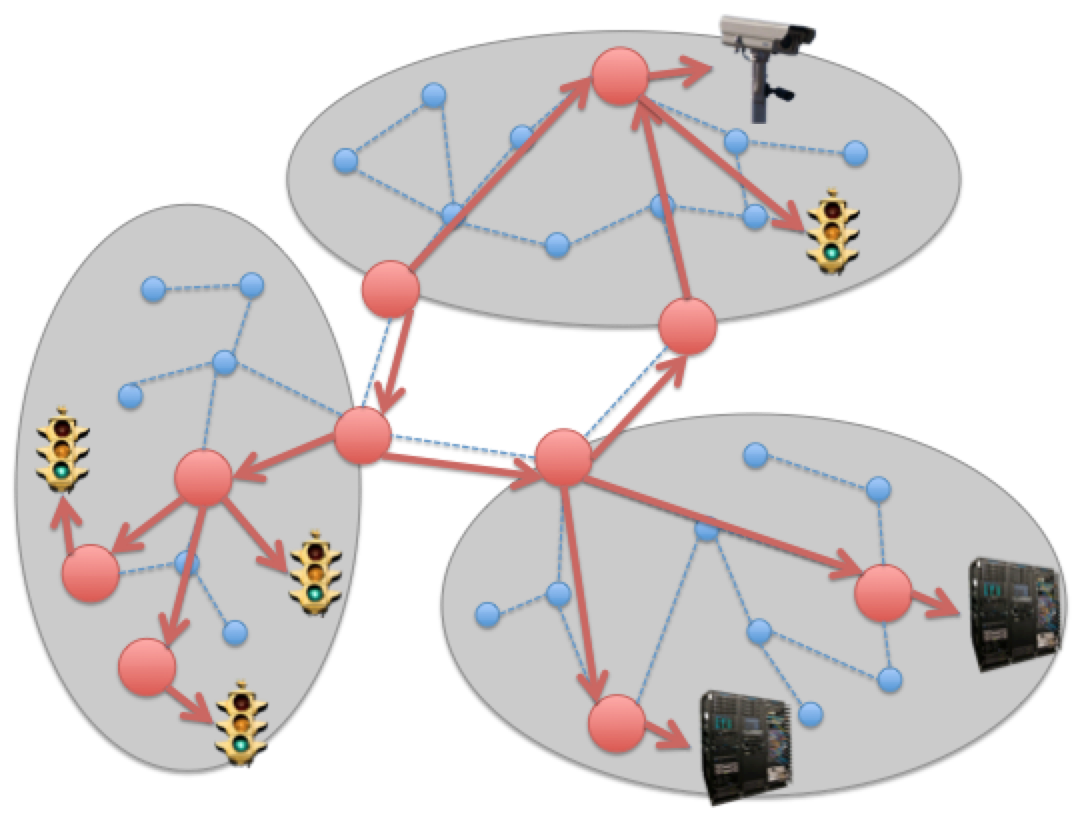
\includegraphics[scale=0.5]{network_example_2}
	\end{center}
	\vspace{-1.2em}
	\caption{\small \itshape An example SCDT running over a physical network with a traffic camera publishing data.  The overlay network  considers only the arrow links, which represent parent-child links.  Legend: large nodes are running SCDT software; small nodes are not running SCDT software; arrow lines are overlay links;  dashed lines are physical links; ovals are trusted domains.}
	\vspace{-1.5em}
	\label{fig:architecture}
\end{figure}

\subsection{Heuristic, Adaptable Multicast}
\label{adaptable-multicast}

SCDTs rely on constructing overlay multicast trees to distribute data to
large numbers of end-devices.  We show an example in~\autoref{fig:architecture}, a 
``smart city" \cite{smart-city}
deployment where street cameras must coordinate with traffic lights at the same
intersection, traffic lights of neighboring intersections, and central servers
far away.  While~\autoref{fig:architecture} only shows a half-dozen end devices, 
the analogy holds
for thousands of end-devices across a smart city, including all traffic lights,
crosswalks, and public transit systems.  Building multicast trees on top of
overlay networks has received significant study in the past \cite{overcast,
	scribe, RFC3208}.  However, these protocols often have questionable scalability, require significant work at the root of the tree, require IP multicast to be running underneath, or disregard latency or security concerns.

Building optimal multicast trees would require unrealistic amounts of overhead
at the scale we are considering.  Instead, SCDTs use heuristic methods.  We describe the characteristics necessary for an IoT
multicast tree building protocol with some similarity to that in
\cite{overcast}, but with several critical modifications.  Subscribers (and
routers serving subscribers) attach to a nearby node in the SCDT and
migrate up or down the tree to best satisfy its latency and bandwidth
constraints.

Unlike many other solutions, we argue for a multicast model in which the
publisher can move in the network and reattach to the SCDT in a different
location.  There are three key benefits to this model.  First, it allows
publishers to be mobile without having to regularly rebuild the entire tree.
Second, it allows nearby nodes (e.g. those with real-time constraints) to
receive data quickly, while still allowing more distant nodes to eventually
receive data.  Third, in the event of a break somewhere up the tree, nearby
devices can still receive data quickly while the tree adapts.  For instance, 
in~\autoref{fig:architecture} a network fault which isolates the local 
intersection from the rest of
the network should not cause interrupt service at the local intersection; instead, while
it may reduce the effectiveness of nearby intersections which are no longer
receiving the data, the local system should continue to function.

We also argue for a publisher/subscriber model in which there is only one
publisher and arbitrarily many subscribers. This greatly simplifies tree
construction and makes it easier to implement a mobile publisher.

End-devices themselves are not the true leaves of the SCDT.  Rather, the routers
these devices connect to should be considered the leaves of the SCDT.  Since
routers are often plugged-in and wired-in, this change in structure allows SCDTs
to impose some processing load on the leaves without compromising low-power or
low-resource devices.  The leaves can determine for themselves when and how
their heterogeneous end-devices should receive data.

Latency should not be disregarded.  Network operators should be able to tune
their devices for a worst case latency before
optimizing for bandwidth.  Latency may even be a more important factor than
bandwidth when considering IoT devices which send data to subscribers relatively
infrequently.  Rather than trying to sample bandwidth, nodes should simply
attach to a nearby parent.  If they are unable to satisfy latency constraints or
keep up with the data stream at their current location, they should migrate
up/down the tree as necessary.  Such a strategy avoids prematurely optimizing
for bandwidth in trees which are only occasionally sending data, and helps to
avoid unnecessarily long, snaking trees.  In~\autoref{fig:architecture}, SCDTs 
provide low latency
to the nearby traffic light which requires current data; meanwhile, devices
further away with looser latency constraints will accrue greater bandwidth
advantages. 

We argue that the optimal metric for ensuring the above properties is \textit{stretch}, introduced in~\autoref{motivation}. 

Rather than considering the Internet as a more or less randomly
distributed graph of nodes, SCDTs consider the network as a series of
interconnected, hierarchical domains of ownership.  Domains are analogous to
Autonomous Systems \cite{RFC1930} and in many cases network operators might
determine domain and AS boundaries to be the same.  Border gateways of
domains/ASes provide a natural choice for multicast points, and can help to
service join requests and maintenance, reducing strain at higher levels of the
SCDT.  While this might provide a single point of failure (or relatively few
points of failure), if the border gateways of an AS fail then there is no access to the
broader Internet anyway.  See~\autoref{domains} for a discussion of the security aspects of domains.

\begin{figure}[t]
	\begin{center}
		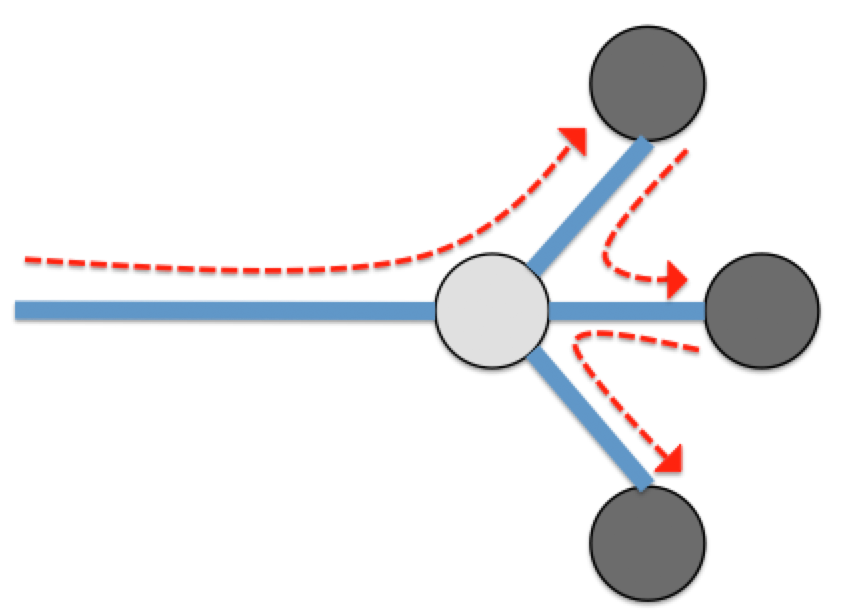
\includegraphics[scale=0.5]{poor_routing.png}
		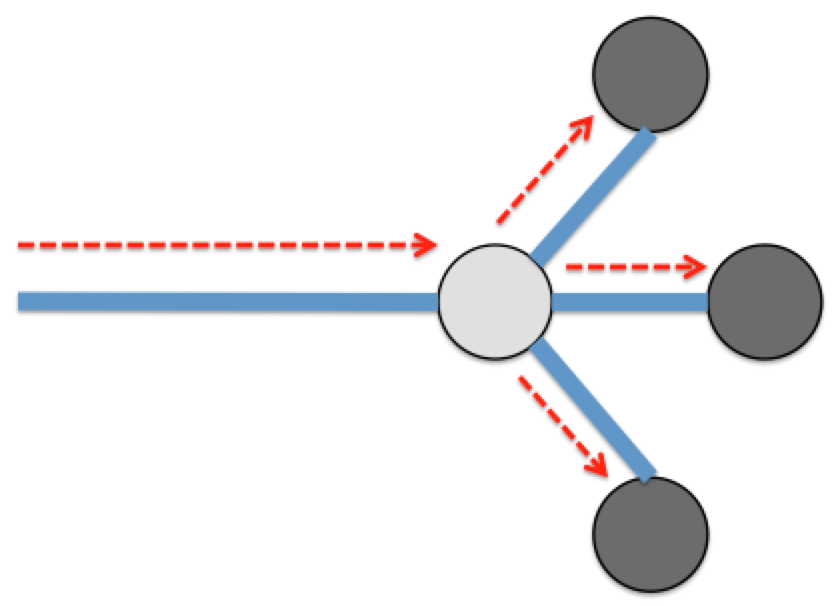
\includegraphics[scale=0.5]{good_routing.png}
	\end{center}
	\vspace{-1.3em}
	\caption{\small \itshape Left: Overlay routing without forced participation, requiring unnecessary retransmission.  Right: Overlay routing with forced participation.  Children receive the packet faster, and the non-subscribing router handles fewer packets.  Legend: light gray routers are not subscribing; dark gray routers are subscribing; solid lines are physical links; dashed lines show packet flow.}
	\vspace{-1em}
	\label{fig:overlay-tree}
\end{figure}

We argue that overlay network routers that are not themselves subscribers to the
data on a particular SCDT should be eligible to be drafted into service to
increase tree efficiency. ~\autoref{fig:overlay-tree} demonstrates a simple 
scenario in which
router promotion would improve routing efficiency.  By analyzing the way overlay
links are constructed over the physical network, the SCDT can identify router
promotions which would increase efficiency.  The ability to promote unknown
routers relies on the construction of trusted domains; only routers within the
trusted domain should be eligible for promotion.
\begin{table}
	\begin{center}
		\begin{tabular}{|c|c|c|c|}
			\hline
			& \textbf{SCDT} & \textbf{Overcast} & \textbf{Scribe} \\
			\hline
			\textbf{Locality Metric} & Stretch & Bandwidth & Typically RTT or Hop Count \\
			\hline
			\textbf{Re-Optimizes Routes} & Yes & Yes & No \\
			\hline
			\textbf{Mobile Publisher} & Yes & No & No \\
			\hline
		\end{tabular}
	\end{center}
	\caption{Comparison of various overlay multicast schemes.}
\end{table}

\subsection{Secure Resolution Systems}
\label{sec-resolution-system}

A key construct of the SCDT system is the Secure Resolution System (SRS)
provided by each domain.  SRSes are roughly analogous to DNS, in that they are a
hierarchical address resolution scheme.  A new subscriber can contact its local
SRS for information on border routers and attachments points for the desired
SCDT.  If the subscriber is the first in its domain, the SRS will point it to
another SRS higher up the hierarchy.

Having all subscribers join the tree by contacting the root is cumbersome and slow. However, because SCDTs involve migrating between attachment points, new subscribers could theoretically use any existing node to join the tree. The closer the initially contacted node is to the ultimate attachment point, the more quickly the SCDT will converge to an optimal placement. The SRSes provide a simple way to find good attach points while allowing local administrators to configure the joining process if necessary. For instance, the local administrator might designate a single node as the domain attach point under the assumption that the domain will always keep that node running; or the administrator could configure a dynamic response based on the knowledge the SRS has about currently active nodes in the domain.

The implementation of the SRS is up to the domain administrator.  A basic version on an SRS could simply be a database on a single server that contains border router information and pointers to other SRSes up the
hierarchy; the IP address of this server could then be hard coded into all
devices in the domain.  A better version could be built using a Distributed Hash
Table \cite{chord, tapestry}.

\subsection{Durability and Replication}
\label{durability-replication}

While many IoT applications involve sending data for immediate consumption, it is also necessary to maintain a store of records somewhere in the network.  The reasons for supporting such replicated, durable storage are threefold.  First, end-devices which require reliable service need a final ground-truth to consult when data has already been completely purged from network caches.  This is also the case for end-devices which go down and come back up later and need to consult data long forgotten by the routing infrastructure or even the publisher itself.  Second, many users will be interested in using analytics to derive insights from historical data.  Third, some devices may only need certain pieces of data, and do not want to be fully joined to the SCDT.

Ideally, the SCDT can perform double duty, transporting data to interested end-devices as well as these ground-truth durable replicas.

\subsection{Mobile Writer}
\label{mobile-writer}
\begin{figure}[t]
	\begin{center}
		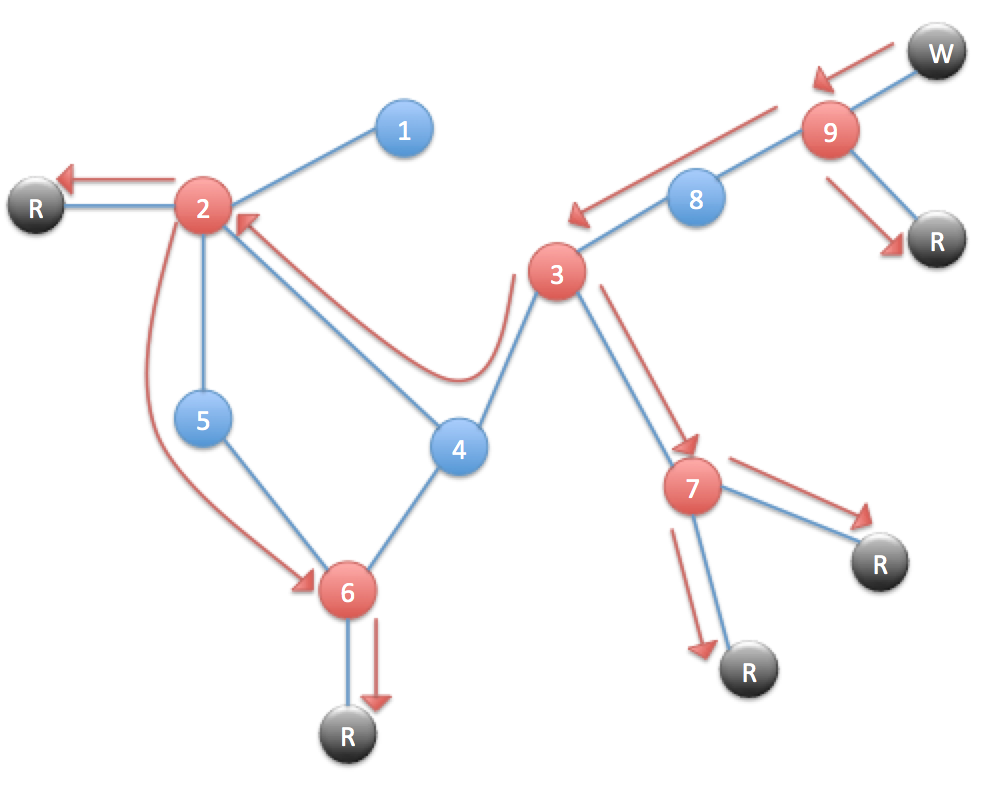
\includegraphics[scale=0.5]{physical_network.png}
		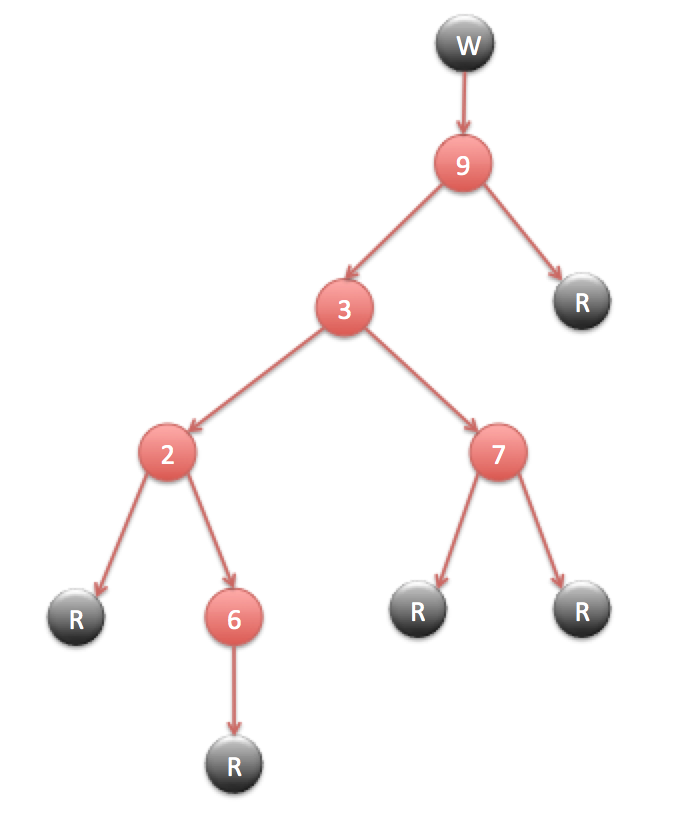
\includegraphics[scale=0.5]{overlay.png}
	\end{center}
	\vspace{-1.3em}
	\caption{\small \itshape Left: A physical network with SCDT nodes running on some machines.  Right: The logical tree formed from that network.  Legend: blue routers are not subscribing; red routers are subscribing; solid lines are physical links; dashed lines show packet flow.}
	\vspace{-1em}
	\label{fig:multicast-tree}
\end{figure}
We have designed SCDTs with a mobile publisher in mind. This means that a self-driving car or robot can reattach to the network elsewhere in the tree quickly. When the publisher rejoins the tree, routers can easily convert their previous parent connection to a child connection (since they're now receiving data from somewhere else). As the receivers continuously test their connections and migrate to better positions, the tree will eventually reform to a shape that better reflects the publisher's new position. The SCDT tree building protocol is extremely lightweight, allowing trees to quickly reform.

\section{Security Implications}
\subsection{Denial of Service}
\label{denial-of-service}
Denial of service and amplification attacks are a major risk in SCDTs, since packets injected into the network will be rebroadcast.  SCDTs are named using a secure namespace that allows many different SCDTs to coexist; specifically, they are named using a cryptographic hash over the credentials of the creator of the tree, making trees attributable to owners and difficult to impersonate.  Subscribers must present a certificate to join the SCDT, which can be verified at the join point, limiting the ability of attackers to attempt to spam the tree or eavesdrop on traffic.  As discussed in~\autoref{adaptable-multicast}, we argue the use of trusted domains to restrict the open flow of data further reduces the risk of data exposure via side channel attacks.  Additionally, the publisher signs data sent to the tree; packets without a valid signature will not be forwarded.  

\subsection{Broadcast Encryption Schemes}
\label{encryption-security}

To achieve confidentiality efficiently, we argue SCDTs should utilize broadcast encryption techniques.  Broadcast encryption \cite{broadcastenc} schemes, such as Subset Difference \cite{subset} or Layered Subset Difference \cite{lsd}, allow data to be efficiently encrypted and transmitted to a large number of receivers securely.  In addition, the publisher can quickly revoke access from misbehaving subscribers by transmitting a limited number of update messages.

\subsection{Trust Domains}
\label{domains}

Domains are a concept introduced by the GDP. A key feature of domains is trust (or lack thereof), primarily based
on domain ownership, so that domains can serve as the boundaries within which
data flows relatively freely.  Organizations can then choose acceptable
domains for their data to flow over, limiting data exposure risks. In order to transit further, developers must either trust other domains (e.g. their ISP) or establish highly secured channels between the border gateways of trusted domains. In many cases, ASes already fit the bill of trusted domains, so few modifications would be necessary to support SCDTs, but domains can also be much more specific, such as in the smart-home example. A simple example of the motivations for trust domains is a smart-home where input device commands must be sent to devices in the same home, but allowing those commands to leave the smart-home risks leaking important information, such as when a user comes and goes.  

A more complicated network might involve a company's office infrastructure in one domain of trust, the company's factory in the next town in a second, and the company's ISP in a third. By grouping the underlying infrastructure into domains of trust, users can specify the flow of data in their networks, simplifying the process of securing data. This method helps to prevent side-channel attacks and other attempts to surreptitiously access encrypted data. For instance, previous research \cite{sidechannel} has shown that analyzing the encrypted traffic of MapReduce jobs can reveal substantial amounts of the supposedly-secure data.

In our previous case, the company could restrict data flow based on their needs by specifying which domains they trust for which data. For example, door open/close notifications may only ever need to be routed to the on-site security staff, and could be restricted from flowing to the ISP, preventing a malicious actor outside the corporate network from learning the comings and goings of employees. The factory might enforce that commands sent to robots on the factory floor cannot flow outside the building to prevent leakage of sensitive information about the manufacturing process. However, the company may mark its ISP's domain as trustworthy for high-level analytics data to move from the factory to the company's offices. 

\section{Evaluation}
\label{scdt-eval}
SCDTs primary differentiator from existing multicast schemes is the application of the stretch metric as the primary component for tree building. Trees are built by new nodes contacting the root, and then moving down the tree to the child that has the best stretch; the process continues until the joining node cannot move further down the tree without exceeding \texttt{MAX\_STRETCH}. An example of a generated overlay topology is shown in~\autoref{fig:topology}. More details can be found in~\autoref{sim-scdt}.

The goal of this metric is construct a tree that balances the need to fan out further down the tree for improve scalability with the real-time or near-real-time requirements of nearby IoT devices. Existing solutions do not take these real-time requirements into account. This solution is also more fault tolerant: partitions in the network, including losing connection to the broader Internet, will not prevent nodes on the same side of the partition as the publisher from continuing to receive content. Existing pub/sub architectures like RabbitMQ and Kafka are focused on the datacenter, and are not designed to account for device locality.

\begin{figure}[h]
	\begin{center}
		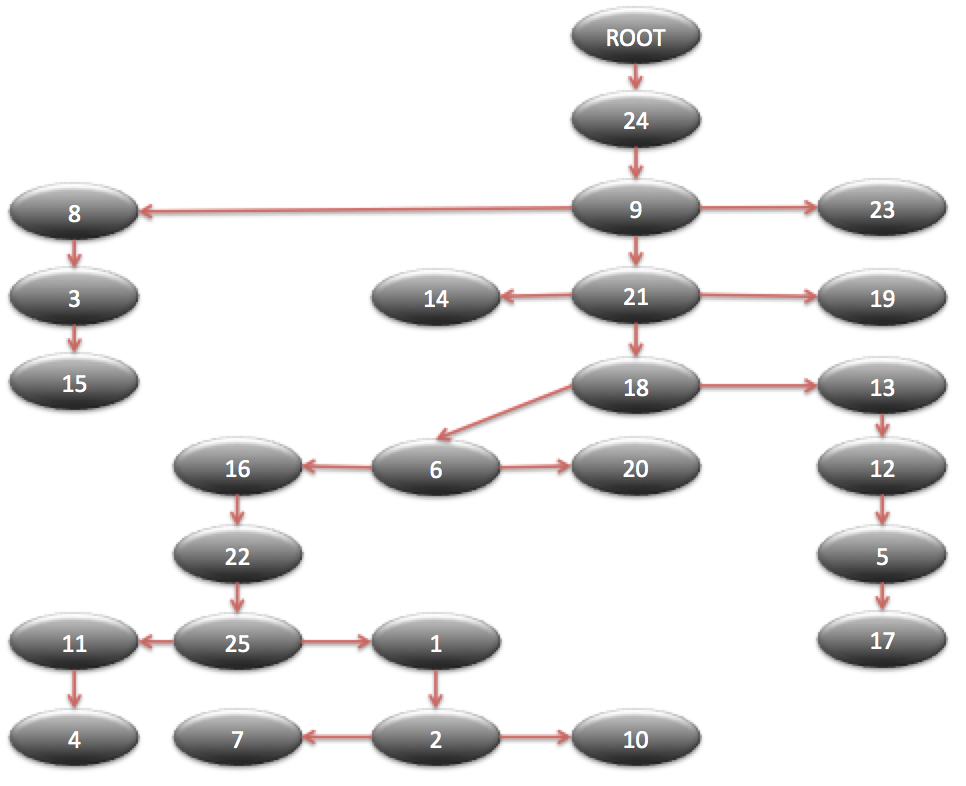
\includegraphics[scale=0.6]{topology.png}
	\end{center}
	\vspace{-1.3em}
	\caption{\small \itshape The overlay multicast tree constructed out of 25 subscriber nodes and 1 publisher connected to a BRITE topology. Topologies vary from run to run due to the randomization of the BRITE topology and the link qualities.}
	\vspace{-1em}
	\label{fig:topology}
\end{figure}

We simulated the impact of using SCDTs to distribute data. Our tests were constructed by generating a BRITE \cite{brite} topology consisting of two connected autonomous systems, and attaching SCDT nodes at the leaves of these ASes.  BRITE topologies are regenerated for each run, helping to eliminate the effect of particular topologies skewing our results.  See~\autoref{simulations} for more details. Link speeds are randomized to between 1 and 10 Mbps, and delays are randomized to between 1 and 50 ms.

\begin{figure}[h]
	\begin{center}
		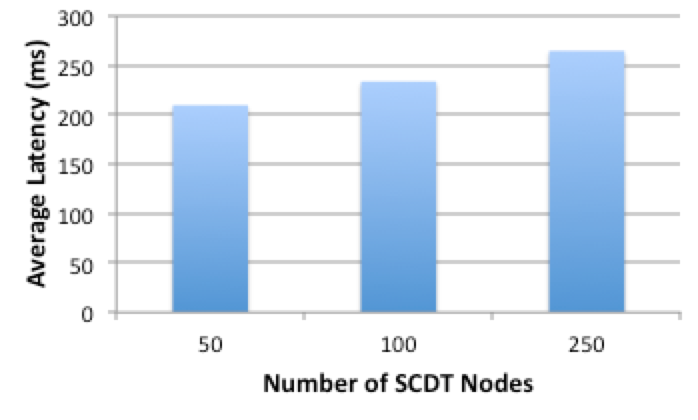
\includegraphics[scale=0.6]{latency_nodes_bar.png}
		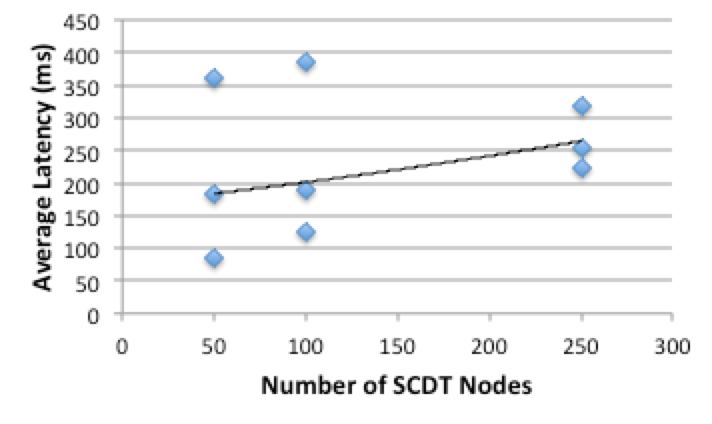
\includegraphics[scale=0.6]{latency_nodes_scat.png}
	\end{center}
	\vspace{-1.3em}
	\caption{\small \itshape Impact on latency of increasing the number of subscribers in the tree, with \texttt{MAX\_STRETCH} set to 2. Left: The average latency of a single packet to subscribers over multiple runs. Right: The average latency of a single packet to subscribers, plotting individual runs and an exponential trend line.}
	\vspace{-1em}
	\label{fig:latency_nodes}
\end{figure}

~\autoref{fig:latency_nodes} demonstrates a test in which a packet is distributed to all SCDT subscribers and average latency is recorded. The latency subscribers encounter appears to increase linearly with the number of nodes in the tree, demonstrating the scale potential of SCDTs. However, we believe results in real-world deployments could scale even further. In our tests, nodes are randomly distributed; in reality, we would be more likely to see node clusters. In some of our tests, random distribution of nodes created a bottlenecking effect, with many nodes attaching to a single point; an intelligently constructed deployment could mitigate that issue.

\begin{figure}[h]
	\begin{center}
		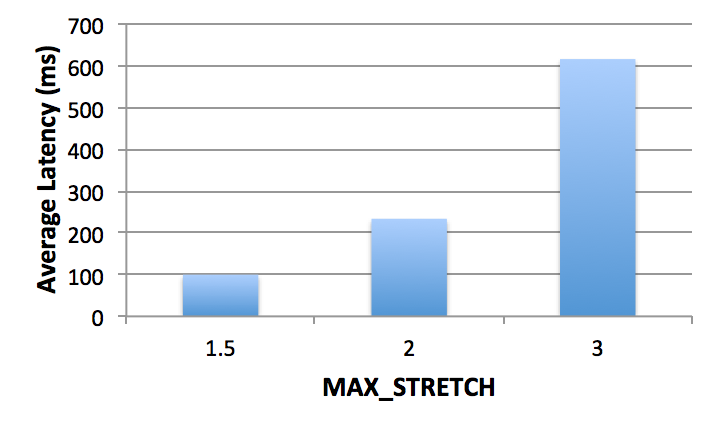
\includegraphics[scale=0.6]{latency_stretch_bar.png}
		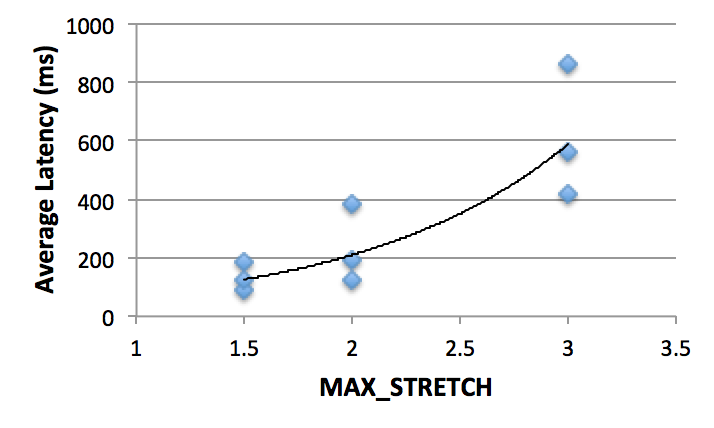
\includegraphics[scale=0.6]{latency_stretch_scat.png}
	\end{center}
	\vspace{-1.3em}
	\caption{\small \itshape Impact on latency of increasing the \texttt{MAX\_STRETCH} parameter in the tree, with the number of subscribers fixed at 100. Left: The average latency of a single packet to subscribers over multiple runs. Right: The average latency of a single packet to subscribers, plotting individual runs and an exponential trend line.}
	\vspace{-1em}
	\label{fig:stretch_nodes}
\end{figure}

We also tested the stretch metric which is at the core of our algorithm. Figure~\autoref{fig:stretch_nodes}, shows the results of these tests. Based on this data, we believe the sweet spot for \texttt{MAX\_STRETCH} tends to be between 1.5 and 2. Lower values had a tendency to severely limit node movement in the tree, resulting in nodes near the top of the tree with a large number of direct children. Our results indicate that as \texttt{MAX\_STRETCH} is increased beyond 2, latency increases at an exponential rate. Examination of some of the constructed trees indicates an excessively high \texttt{MAX\_STRETCH} leads to long, snaking trees with limited branching.

~\autoref{fig:stretch_nodes} is also important for establishing the efficiency of SCDTs over other schemes.  The case where \texttt{MAX\_STRETCH} is set to one degenerates into a unicast relationship between the root and all children. This is obviously not a tenable situation as the trees continue to scale, but even at 100 nodes, SCDTs are about 30\% faster than the basic unicast case with \texttt{MAX\_STRETCH} is set to 1.5.

\begin{figure}[h]
	\begin{center}
		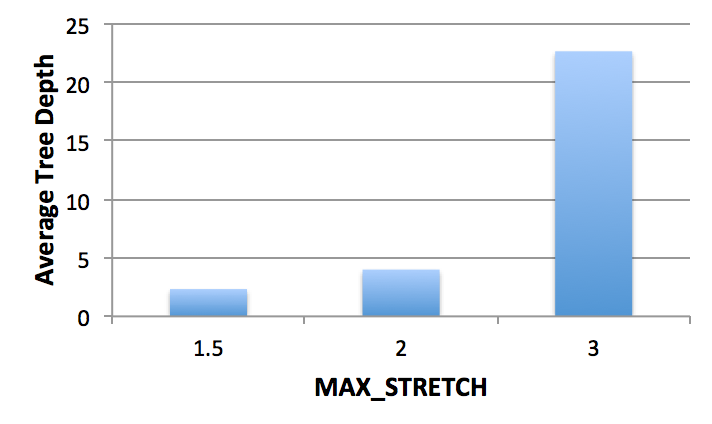
\includegraphics[scale=0.6]{depth_stretch_bar.png}
		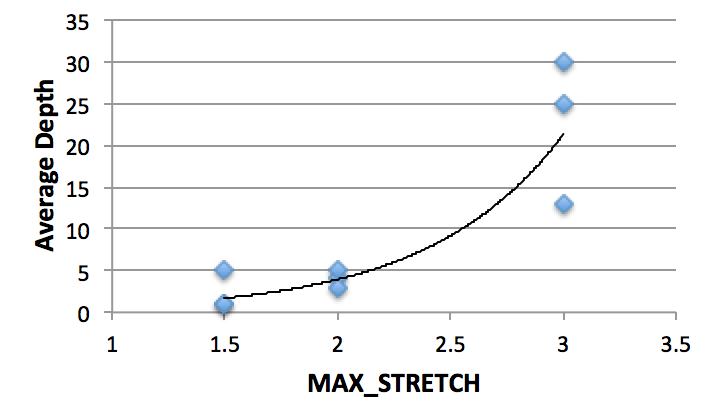
\includegraphics[scale=0.6]{depth_stretch_scat.png}
	\end{center}
	\vspace{-1.3em}
	\caption{\small \itshape Impact on tree depth of increasing the \texttt{MAX\_STRETCH} parameter in the tree, with the number of subscribers fixed at 100. Left: The average depth of the tree over multiple runs. Right: The average depth of the tree plotting individual runs and an exponential trend line.}
	\vspace{-1em}
	\label{fig:depth_stretch}
\end{figure}

The results in~\autoref{fig:stretch_nodes} are further reinforced by examining the average depth of nodes in SCDTs, show in~\autoref{fig:depth_stretch}. As expected, tree depth tends to increase exponentially with \texttt{MAX\_STRETCH}, leading to the aforementioned exponential increase in latency.

Our results show that tuning the \texttt{MAX\_STRETCH} parameter for particular deployments will be critical. SCDTs, however, do allow a large degree of flexibility. The \texttt{MAX\_STRETCH} value is set at the node level, not the network level, meaning that every node could have its own individually-tailored \texttt{MAX\_STRETCH}.

This is an important property for real-world deployments. \texttt{MAX\_STRETCH} could be set based on device priority; real-time applications could enforce a lower \texttt{MAX\_STRETCH} while batch processing applications could settle for a much higher \texttt{MAX\_STRETCH}.  

It may also be important to tune this parameter based on where nodes (or clusters of nodes) are positioned in the network. Nodes located far from the root may counterintuitively require lower stretch values. These nodes will have a large latency when contacting the root, reducing sensitivity to placement in their local area (see~\autoref{motivation}). This effect could also be offset by introducing intermediate join points in the tree, i.e. nodes that can serve as a proxy for the root, as discussed in~\autoref{sec-resolution-system}.
	
\begin{figure}[h]
	\begin{center}
		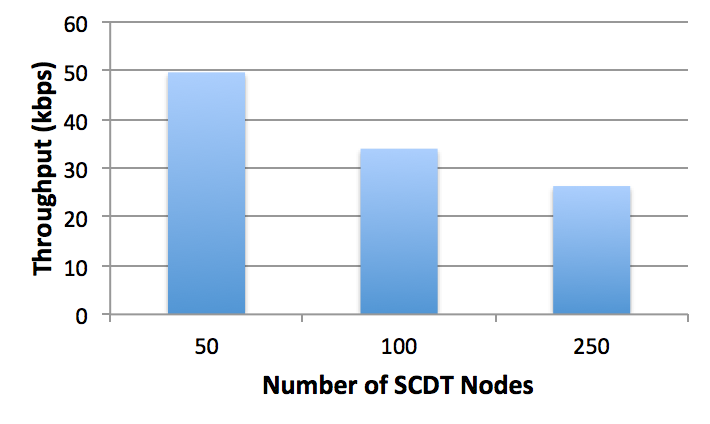
\includegraphics[scale=0.6]{through_nodes_bar.png}
		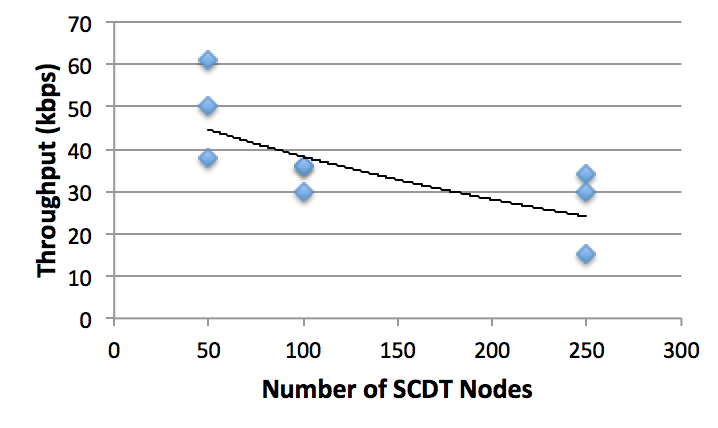
\includegraphics[scale=0.6]{through_nodes_scat.png}
	\end{center}
	\vspace{-1.3em}
	\caption{\small \itshape Impact on throughput of increasing the number of subscribers in the tree. Sampled by sending 10KB with \texttt{MAX\_STRETCH} fixed at 2. Left: The average throughput of the tree over multiple runs. Right: The average throughput of the tree plotting individual runs and an exponential trend line.}
	\vspace{-1em}
	\label{fig:through_nodes}
\end{figure}

Finally, we examine how SCDTs perform in terms of throughput. ~\autoref{fig:through_nodes} shows that average throughput decreases approximately linearly as the number of nodes increases. Note that these values should not be compared to the values in~\autoref{cnr-eval} directly since each test was conducted under different parameters and configurations.  

We also compared SCDTs throughput performance to the naive tree building method used for evaluation in~\autoref{cnr-eval} and described in~\autoref{sim-cnr}. Due to limitations in our simulations, we did not compare these at scale. However, we did compare the naive tree building method, in which each node has a fixed fanout and chooses its children based on latency, on a simulation containing 50 nodes. Throughput comparisons were found to be fairly comparable between the naive implementation at this size.  Latency comparisons were also similar.  While further scaling of these simulations is necessary to prove the effectiveness of SCDTs, we believe these results show that the concept has great promise.

Overall, SCDTs performed well in our tests. Both latency and throughput appear to scale well in our examinations. The most significant challenge is properly tuning the \texttt{MAX\_STRETCH} parameter. However, we have many improvements in mind for SCDTs, which we discuss in~\autoref{future}, which we believe will further improve SCDTs. 